%*******************************************************************************
%****************************** Primo capitolo *********************************
%*******************************************************************************

\chapter{Introduzione}

L’obiettivo di questo progetto è quello di realizzare un veicolo alimentato a batteria in grado di localizzarsi su una mappa preacquisita e di navigare all’interno di essa sfruttando un sensore Lidar ed antenne Ultra-wideband (UWB).

Il motivo della scelta di tali sensori è legato al fatto che il veicolo deve esser capace di localizzarsi in una duplice maniera così da ovviare a fallimenti temporanei di uno dei due sistemi: nello specifico si utilizza il sensore Lidar per eseguire uno scan-matching rispetto alla mappa e si corregge la posa stimata, se necessario, sfruttando le informazioni provenienti dal sistema UWB. 
Infatti, i due metodi di localizzazione sono circa complementari, dato che lo scan-matching, una volta individuata la posizione approssimata nella mappa, è capace di dare stime corrette con elevata precisione, ma può arrivare a perdersi completamente in ambienti troppo poco eterogenei (ad esempio un corridoio lungo e senza riferimenti) o in caso di oscuramento del sensore; è in questo caso che per correggere la stima di posa del robot subentrano le UWB.

%********************************** Sezione 1.1  **************************************
\section{Descrizione del sistema}
\label{section1.1}
L’hardware è composto da un veicolo a quattro ruote dotato di un motore per l'asse posteriore ed uno per l'asse anteriore, sul quale è presente anche un servo che funge da sterzo.
Per quanto riguarda l'elettronica di bordo, sono presenti due unità centrali (vedi Figura~\ref{fig:schema_hardware}):
\begin{itemize}
    \item Un’Intel\textsuperscript\textregistered Joule\texttrademark, con sistema operativo Linux 16.04 su cui viene eseguito Robot Operating System (ROS)
    \item Un microcontrollore STM32F407\textsuperscript\textregistered \hspace{1mm}su cui è implementato il sistema di guida
\end{itemize}

\noindent Oltre a questi, sono presenti:
\begin{itemize}
    \item Un sensore Lidar Slamtec\textsuperscript\textregistered \hspace{1mm}RPLIDAR-A3\texttrademark
    \item Un sistema di localizzazione Ultra-wideband (Pozyx\textsuperscript\textregistered) composto da due tag installate sul veicolo e 4 ancore disposte sul terreno.
\end{itemize}

A livello macroscopico, al modulo Intel\textsuperscript\textregistered Joule\texttrademark \hspace{1mm}è affidato il compito di raccogliere i dati provenienti dal Lidar e dalle tag, e fornire una stima della posa del robot all'interno di una mappa preacquisita; successivamente questa stima viene quindi inviata all’STM\textsuperscript\textregistered, la quale calcola i valori di controllo in pulse-width modulation, PWM, per lo sterzo e l’acceleratore del veicolo affinché venga raggiunto un punto desiderato sulla mappa.

\begin{figure}[h]
\centering    
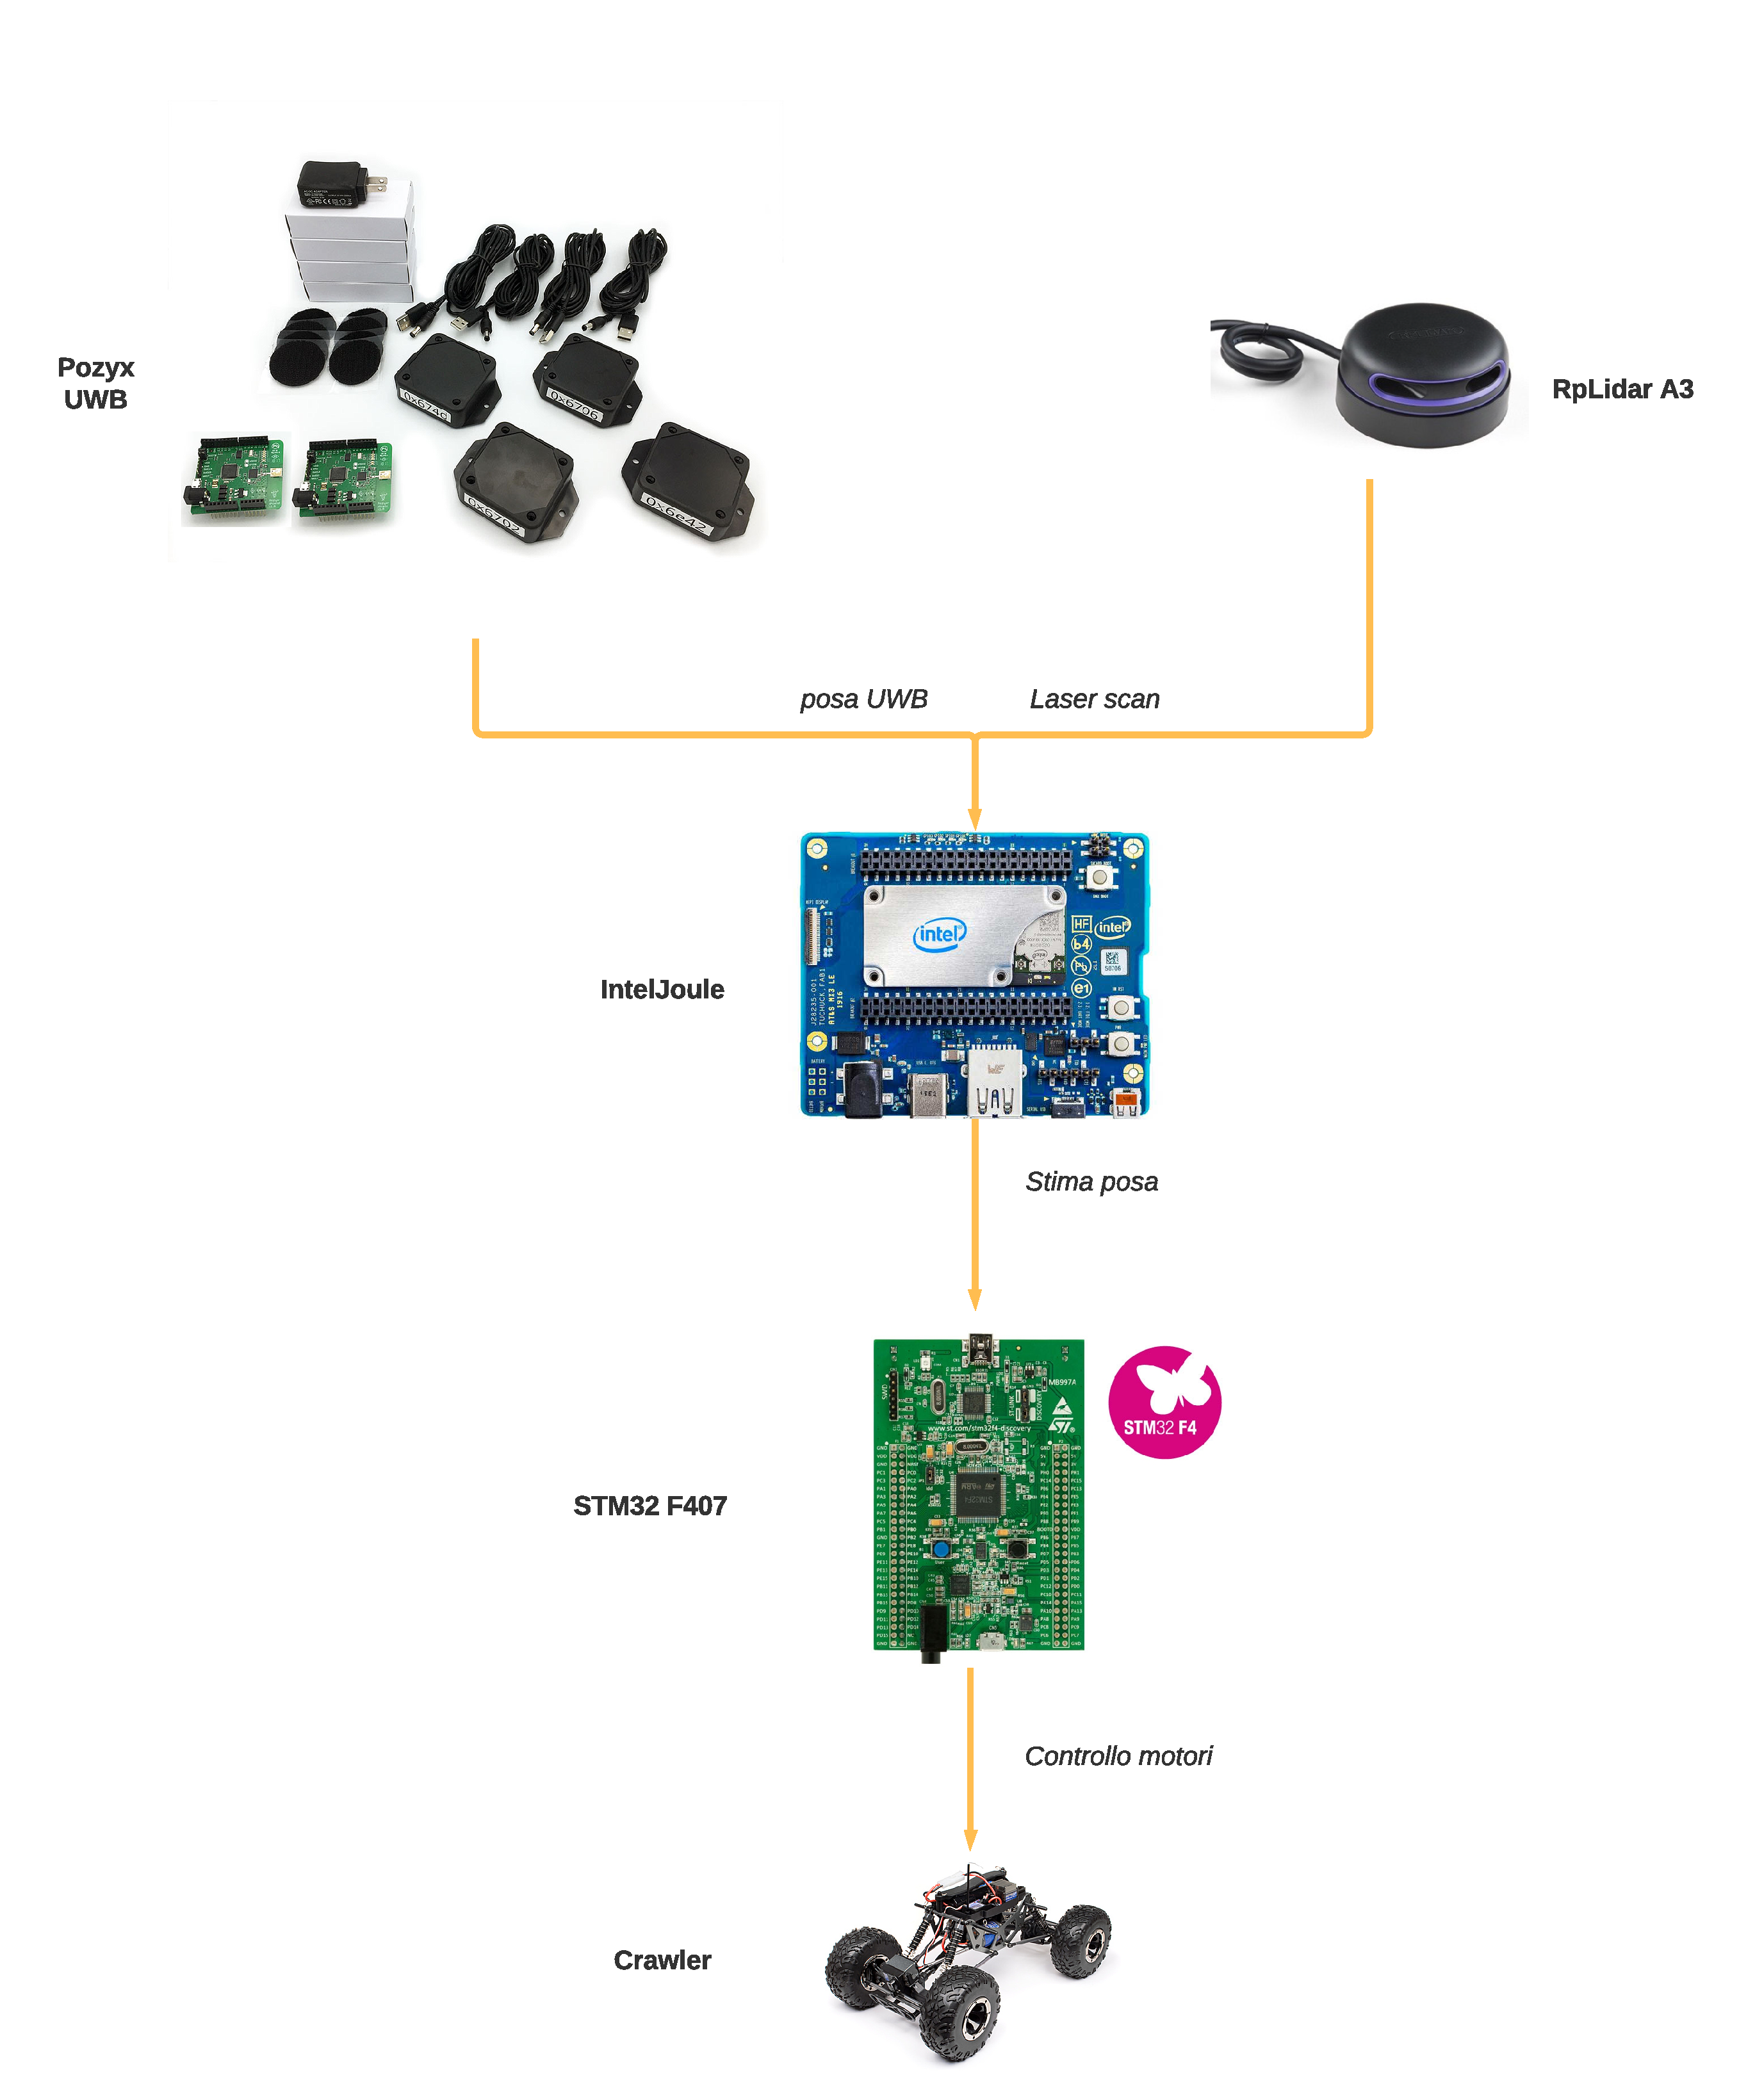
\includegraphics[width=0.77\textwidth]{Capitolo1/Figs/schema_hardware.pdf}
\caption[Schema hardware del veicolo]{Schema hardware del veicolo}
\label{fig:schema_hardware}
\end{figure}

% ********************************** Sezione 1.1.1  **************************************
\subsection{In dettaglio}
\label{subsection1.1.1}

\subsubsection*{Alimentazione}
\label{subsubsection1.1.1.1}

Il robot è dotato di due batterie:
\begin{itemize}
    \item LiPo $14.6$V $4200$mAh, dedicata ad un’alimentazione generica, che viene sfruttata da tutti i componenti tranne i motori; da questa partono 3 linee di alimentazione: 
    \begin{itemize}
        \item a $14.6$V per la STM\textsuperscript\textregistered
        \item a $12$V per la Intel\textsuperscript\textregistered Joule\texttrademark
        \item a 5V per fornire alimentazione ausiliaria all’HUB-USB
    \end{itemize}
    \item LiPo $7.4$V $6000$mAh dedicata ai motori
\end{itemize}

I vari convertitori di tensione sono tutti installati su una PCB, che è posizionata all’interno di un box metallico per schermarne la radiazione elettromagnetica.

\bigskip

\begin{figure}[h] 
\centering    
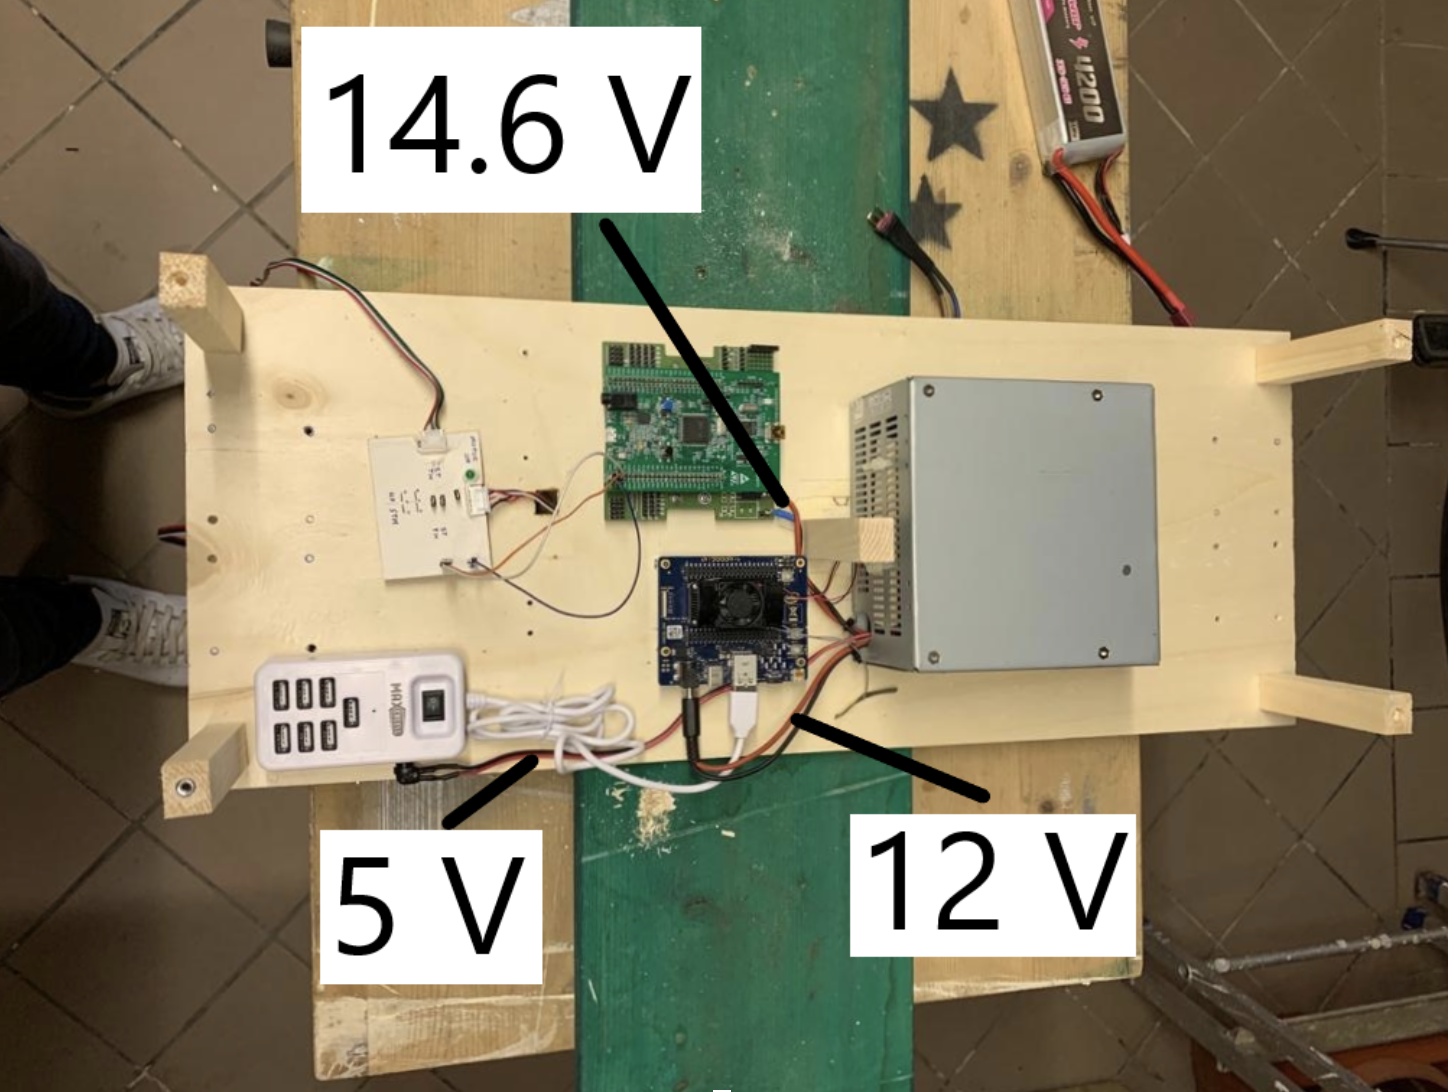
\includegraphics[scale=0.3]{Capitolo1/Figs/batteria.png}
\caption[Alimentazione]{Linee di alimentazioni dalla LiPo 14.6V 4200mAh}
\label{fig:alimentazione}
\end{figure}

\subsubsection*{Connessioni}
\label{subsubsection1.1.1.2}

Sia il Lidar che le due tag UWB sono connesse all’Intel\textsuperscript\textregistered Joule\texttrademark\hspace{1mm}tramite un HUB-USB, oltre a queste è presente un convertitore USB-TTL utilizzato per comunicare con l’STM32F407\textsuperscript\textregistered\hspace{1mm}via seriale. 
Il canale TX del convertitore TTL è connesso al canale RX della porta “UART 5” dell’STM\textsuperscript\textregistered \hspace{1mm}mentre il canale RX del convertitore TTL è connesso al canale TX della porta “UART 2” dell’STM.

\clearpage

\null
\vfill
\textbf{Connessioni in dettaglio tra STM\textsuperscript\textregistered e Motori}

\bigskip

I motori sono alimentati da una batteria LiPo dedicata da $7.4$V $6000$mAh, questa è connessa ad un controller che gestisce i due motori di traino anteriore e posteriore e fornisce alimentazione per il servo. Il controller dispone di una linea di ingresso, che si aspetta un segnale in PWM per regolare la velocità dei motori di traino, mentre il controllo dell’angolo del servo si ha tramite un secondo PWM separato. Lo schema di dettaglio è mostrato in Figura~\ref{fig:stm_motori}.

\begin{figure}[h] 
\centering    
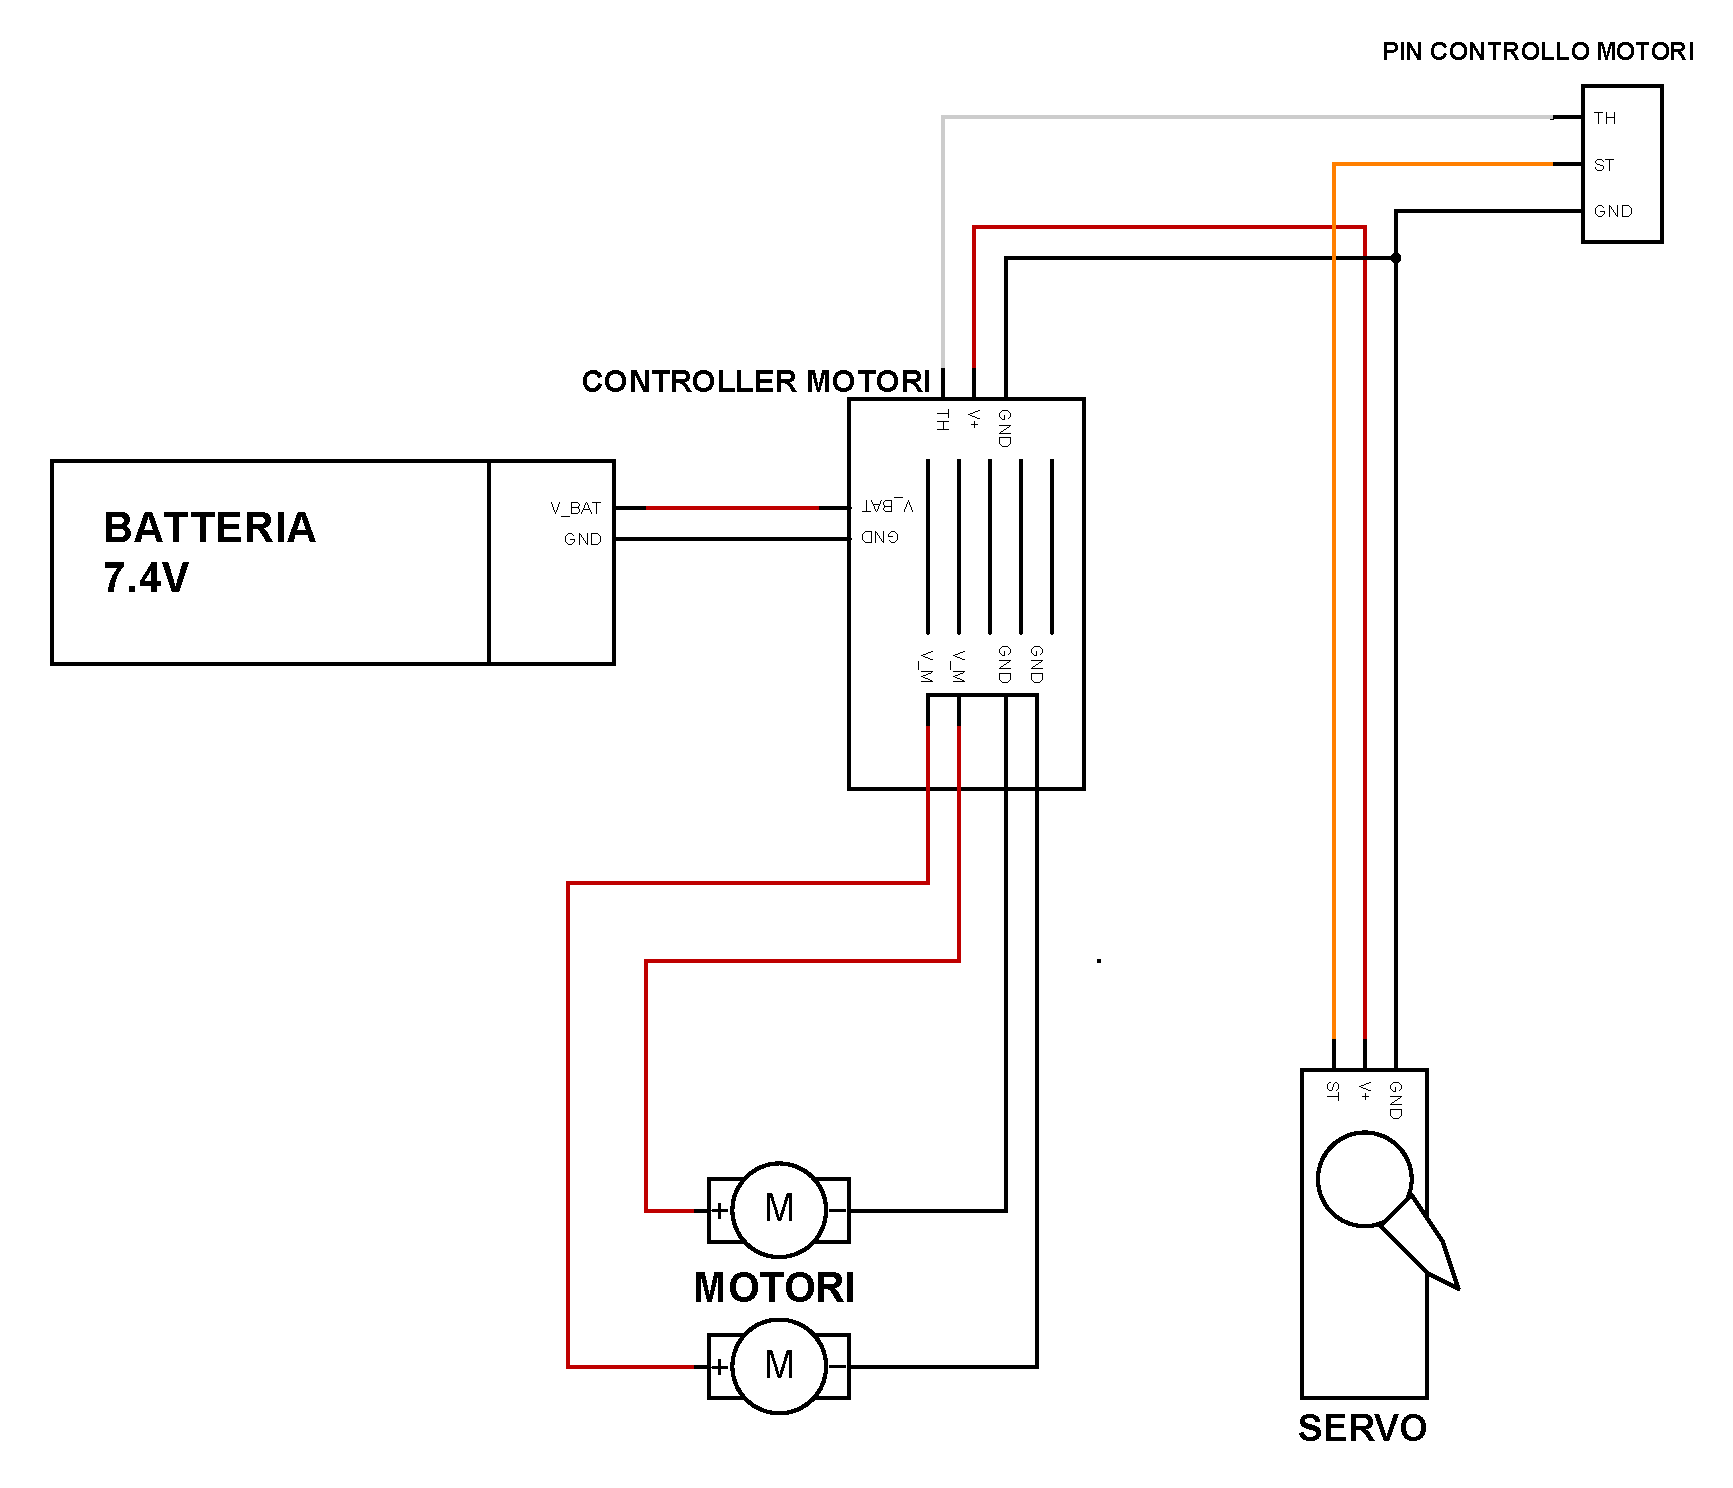
\includegraphics[width=0.89\textwidth]{Capitolo1/Figs/connessioni_stm_motori.pdf}
\caption[Connessioni tra STM\textsuperscript\textregistered e motori]{Connessione tra STM\textsuperscript\textregistered e motori}
\label{fig:stm_motori}
\end{figure}
\vfill

\clearpage

\null
\vfill
\textbf{Connessioni in dettaglio - schema completo}
\bigskip
\begin{figure}[h] 
\centering    
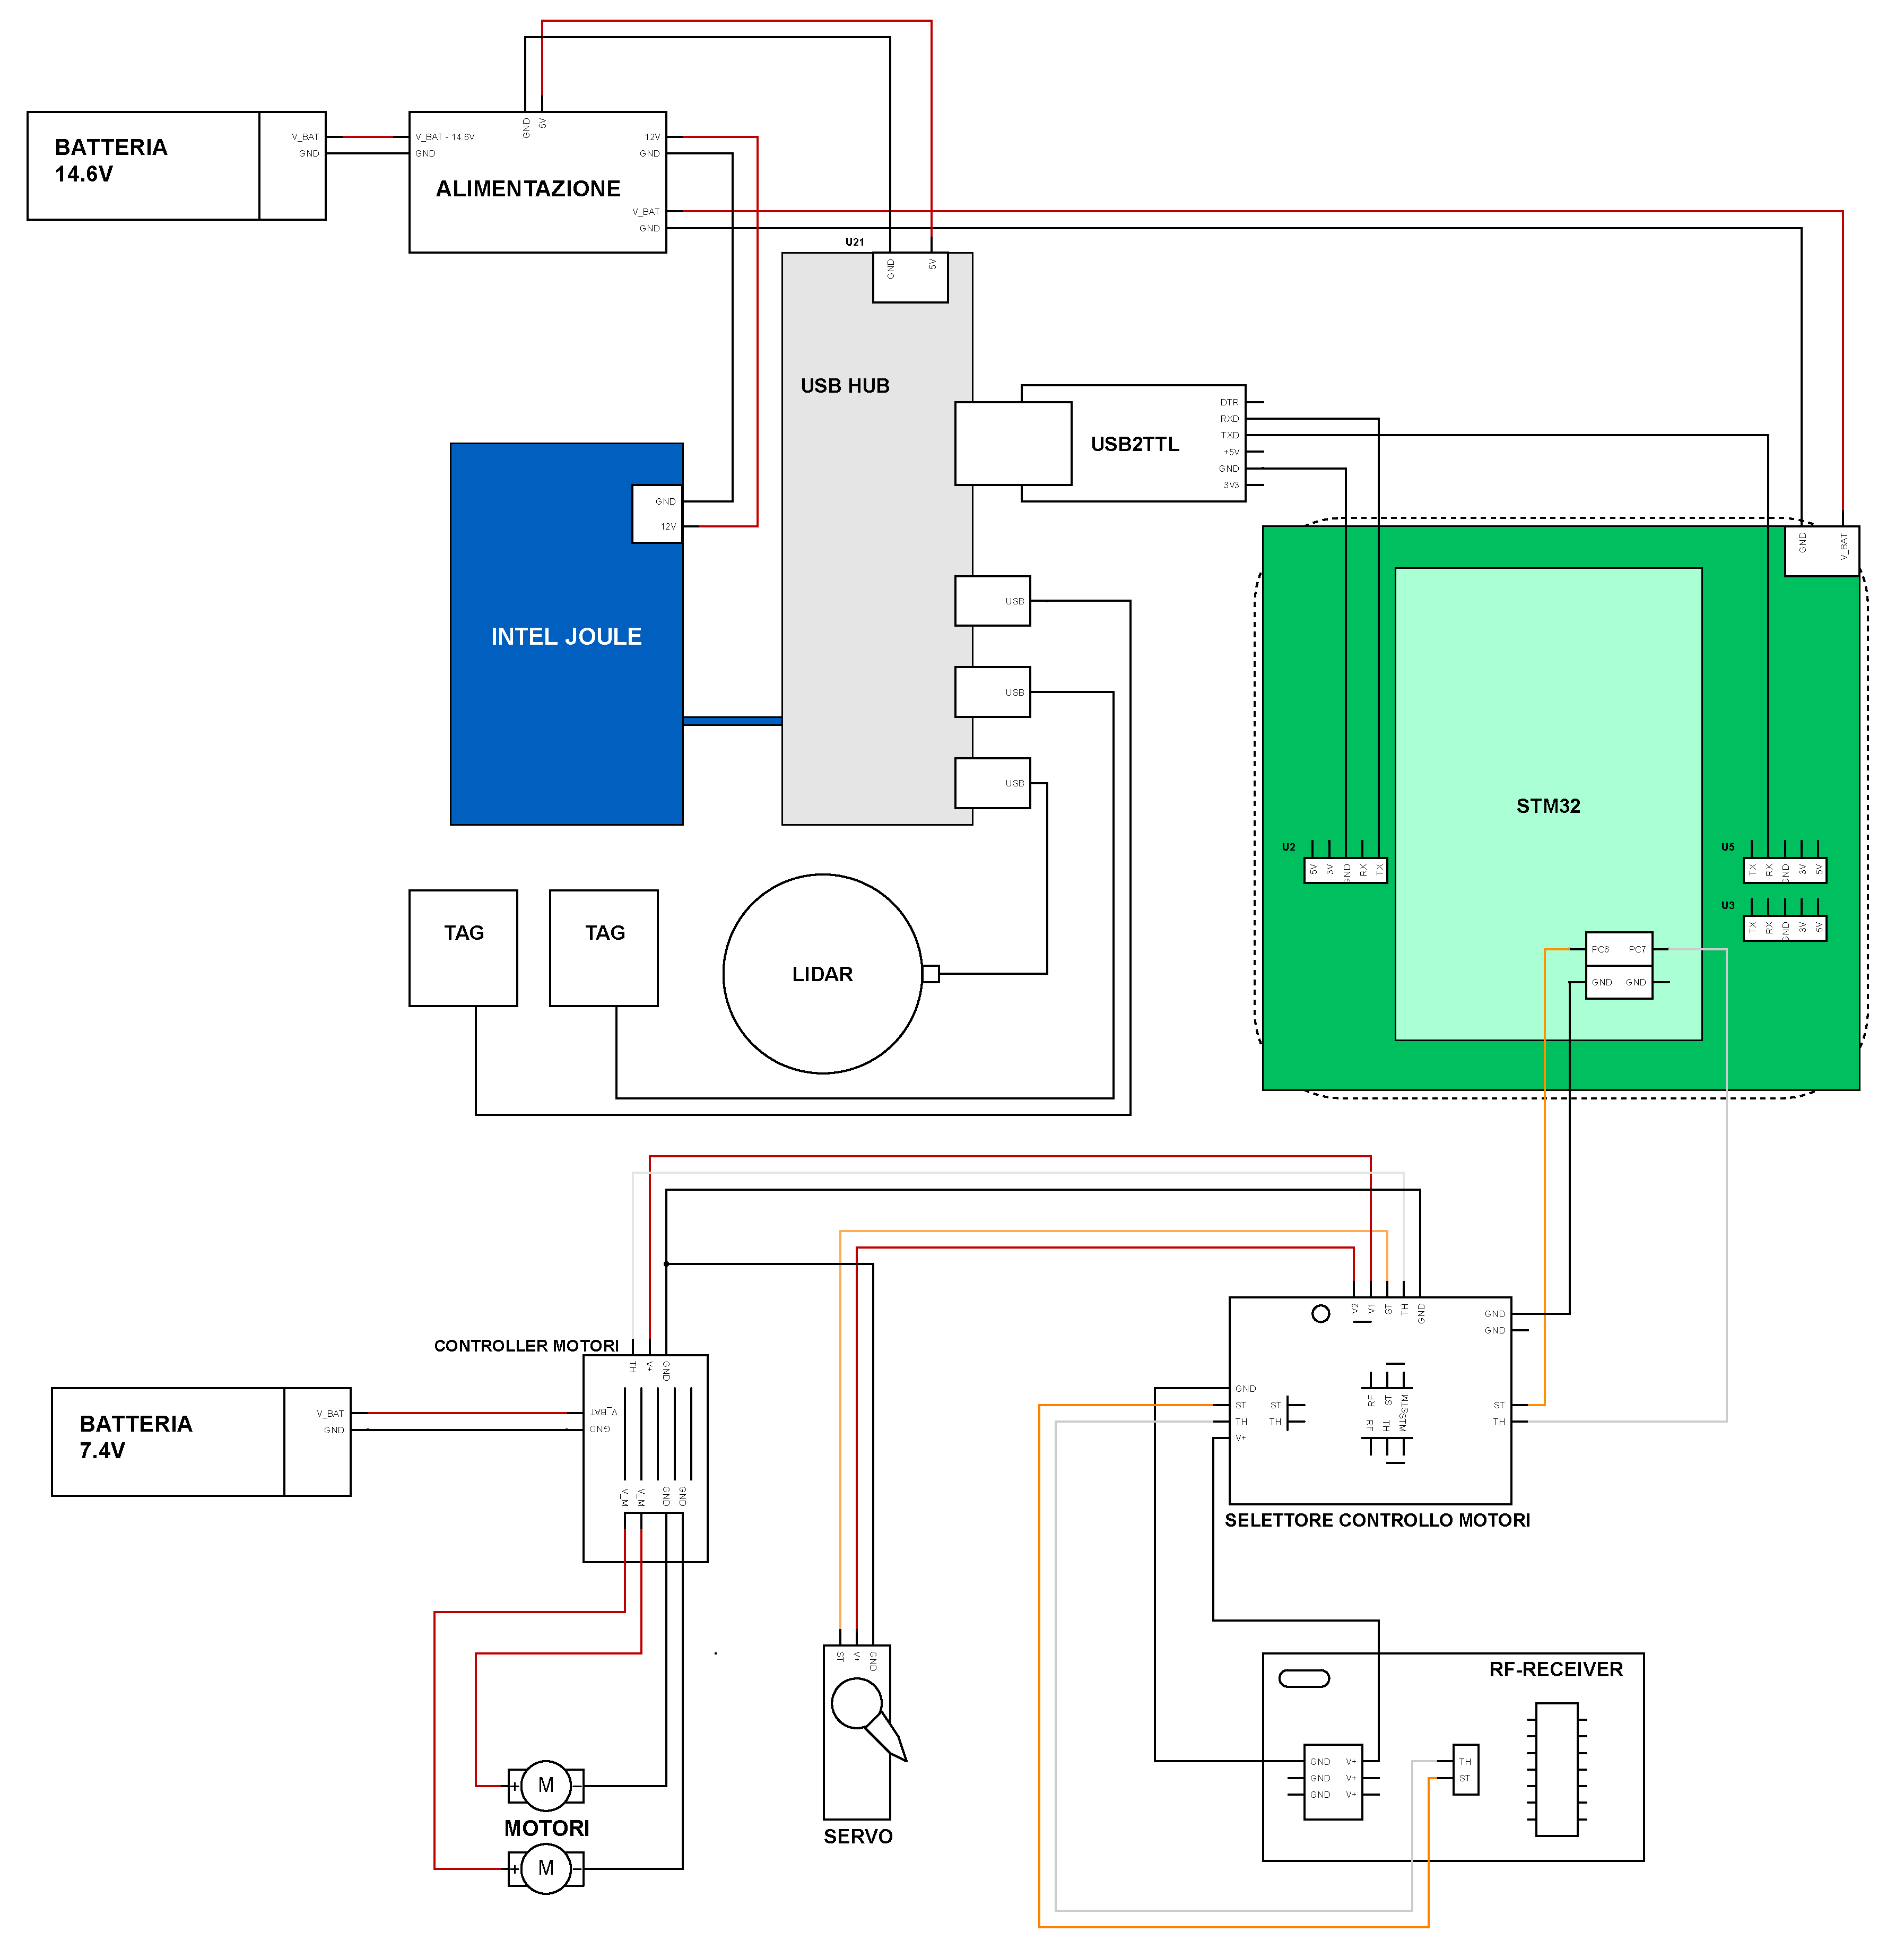
\includegraphics[width=1\textwidth]{Capitolo1/Figs/schema_luca.pdf}
\caption[Schema completo]{Schema completo}
\label{fig:schema_completo}
\end{figure}

\vfill

\clearpage

% ********************************** Sezione 1.2 *************************************
\section{Punto di partenza}
\label{section1.2}
Il veicolo è stato ricevuto come mostrato in Figura~\ref{fig:bipe}.

\noindent Si è provato  riprodurre i passaggi indicati dal gruppo precedente per valutare le condizioni correnti e identificare possibili comportamenti da correggere. 

Dopo averlo ispezionato ed analizzato sono emerse alcune criticità sia a livello hardware sia a livello software e che verranno illustrate nei paragrafi seguenti.

\begin{figure}[h] 
\centering    
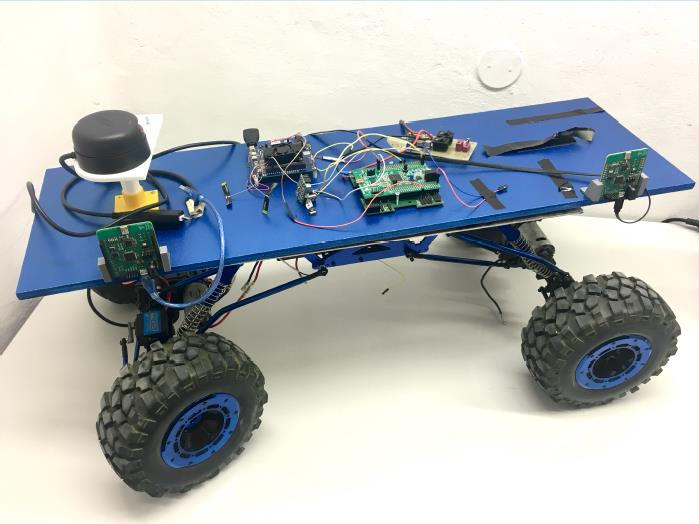
\includegraphics[scale=0.33]{Capitolo1/Figs/bipe.jpg}
\caption[Veicolo ricevuto dal gruppo precedente]{Veicolo di partenza, ricevuto dal gruppo precedente}
\label{fig:bipe}
\end{figure}
% ********************************** % Subsection 1.2.1  *************************************
\subsection{Hardware}
\label{subsection1.2.1}
La prima problematica che è risultata evidente era riguardo la disposizione dell’elettronica sulla tavola in legno. Le schede non erano fissate ed i contatti tra le varie componenti risultavano molto precari. Ciò si traduceva in improvvisi malfunzionamenti o addirittura totali spegnimenti del sistema.

Per quanto riguarda la struttura, le sospensioni non erano in grado di mantenere la tavola con l’elettronica su di un piano orizzontale, ma si aveva un forte cedimento in particolar modo sul lato sinistro del veicolo, che causava un’inclinazione della tavola con conseguente impossibilità per il Lidar di effettuare un match con la mappa, dato che i piani non erano più allineati.

Inoltre, era necessario ripensare la disposizione generale delle varie componenti in modo da mantenere i sensori separati da tutto il resto, avere un maggiore livello di ordine ed anche una disposizione dei pesi più omogenea.

In secondo luogo vi era un problema di sottoalimentazione dei sensori, in particolare del Lidar, che non riceveva sufficiente alimentazione dalla sola porta USB-A della Intel\textsuperscript\textregistered Joule\texttrademark \hspace{1mm}, ciò andava a compromettere i risultati della scansione, che in alcuni casi non era nemmeno in grado di avviarsi.

E’ stato poi riscontrato un problema di interferenza elettromagnetica causato dalla batteria e dall'elettronica switching di alimentazione, che condizionavano in maniera significativa il funzionamento delle tag poste sul veicolo introducendo rumore non trascurabile e salti di posizione con ampiezza fino ad 1m.
% ********************************** % Subsection 1.2.2  *************************************
\subsection{Software}
\label{subsection1.2.2}

A livello software sono stati notati principalmente due problemi:
\begin{enumerate}
    \item Servomotore, il quale non appena avviata la comunicazione seriale con la Intel\textsuperscript\textregistered  \hspace{1mm}Joule\texttrademark \hspace{1mm}iniziava ad avere un comportamento anomalo che consisteva in continui cambi di orientamento delle ruote
    \item Il secondo problema invece si presentava nel publisher di posa delle UWB che era caratterizzato da un numero di fallimenti molto elevato, con un rapporto di circa un fallimento ogni 5 pacchetti inviati correttamente.
\end{enumerate}
%********************************** % Section 1.3  *************************************
\section{Modifiche}
\label{section1.3}

In primis è stato necessario ottenere un sistema robusto ed affidabile su cui effettuare i successivi esperimenti, con questo scopo sono stati installati dei distanziatori su cui sono state avvitate le schede, così da garantirne una posizione ben salda.

\medskip

\begin{figure}[h]
  \centering
  \begin{subfigure}[b]{0.35\textwidth}
    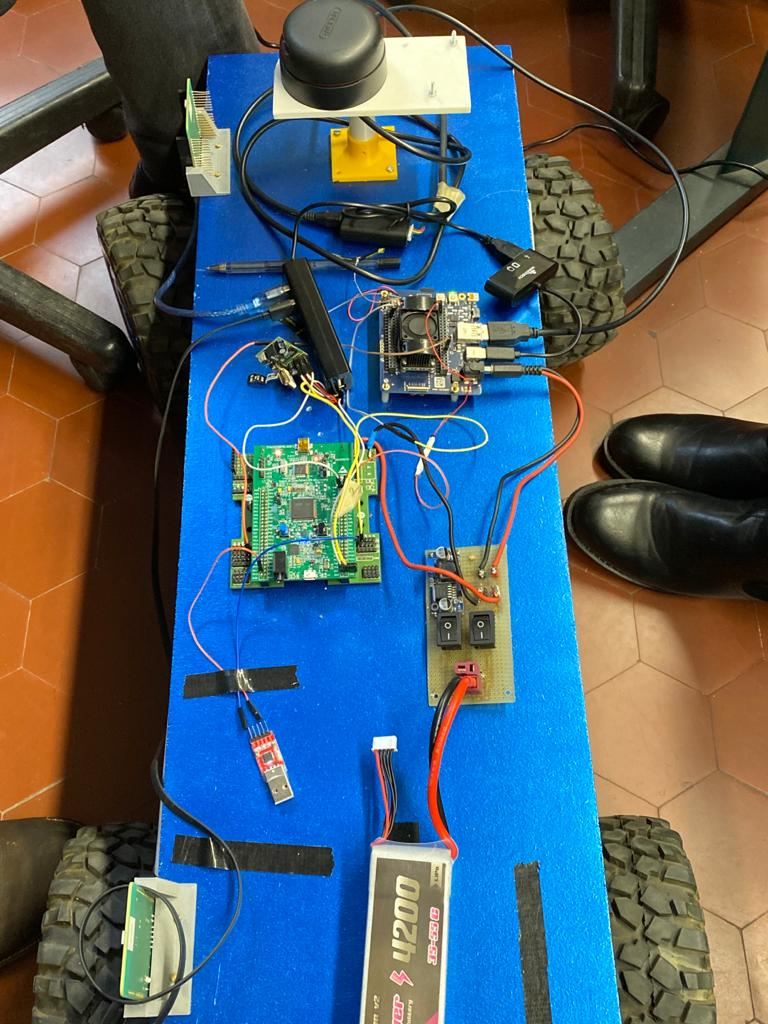
\includegraphics[width=\textwidth]{Capitolo1/Figs/foto_prima.png}
    \caption{Foto prima}
    \label{fig:foto_prima}   
  \end{subfigure}             
  \begin{subfigure}[b]{0.35\textwidth}
    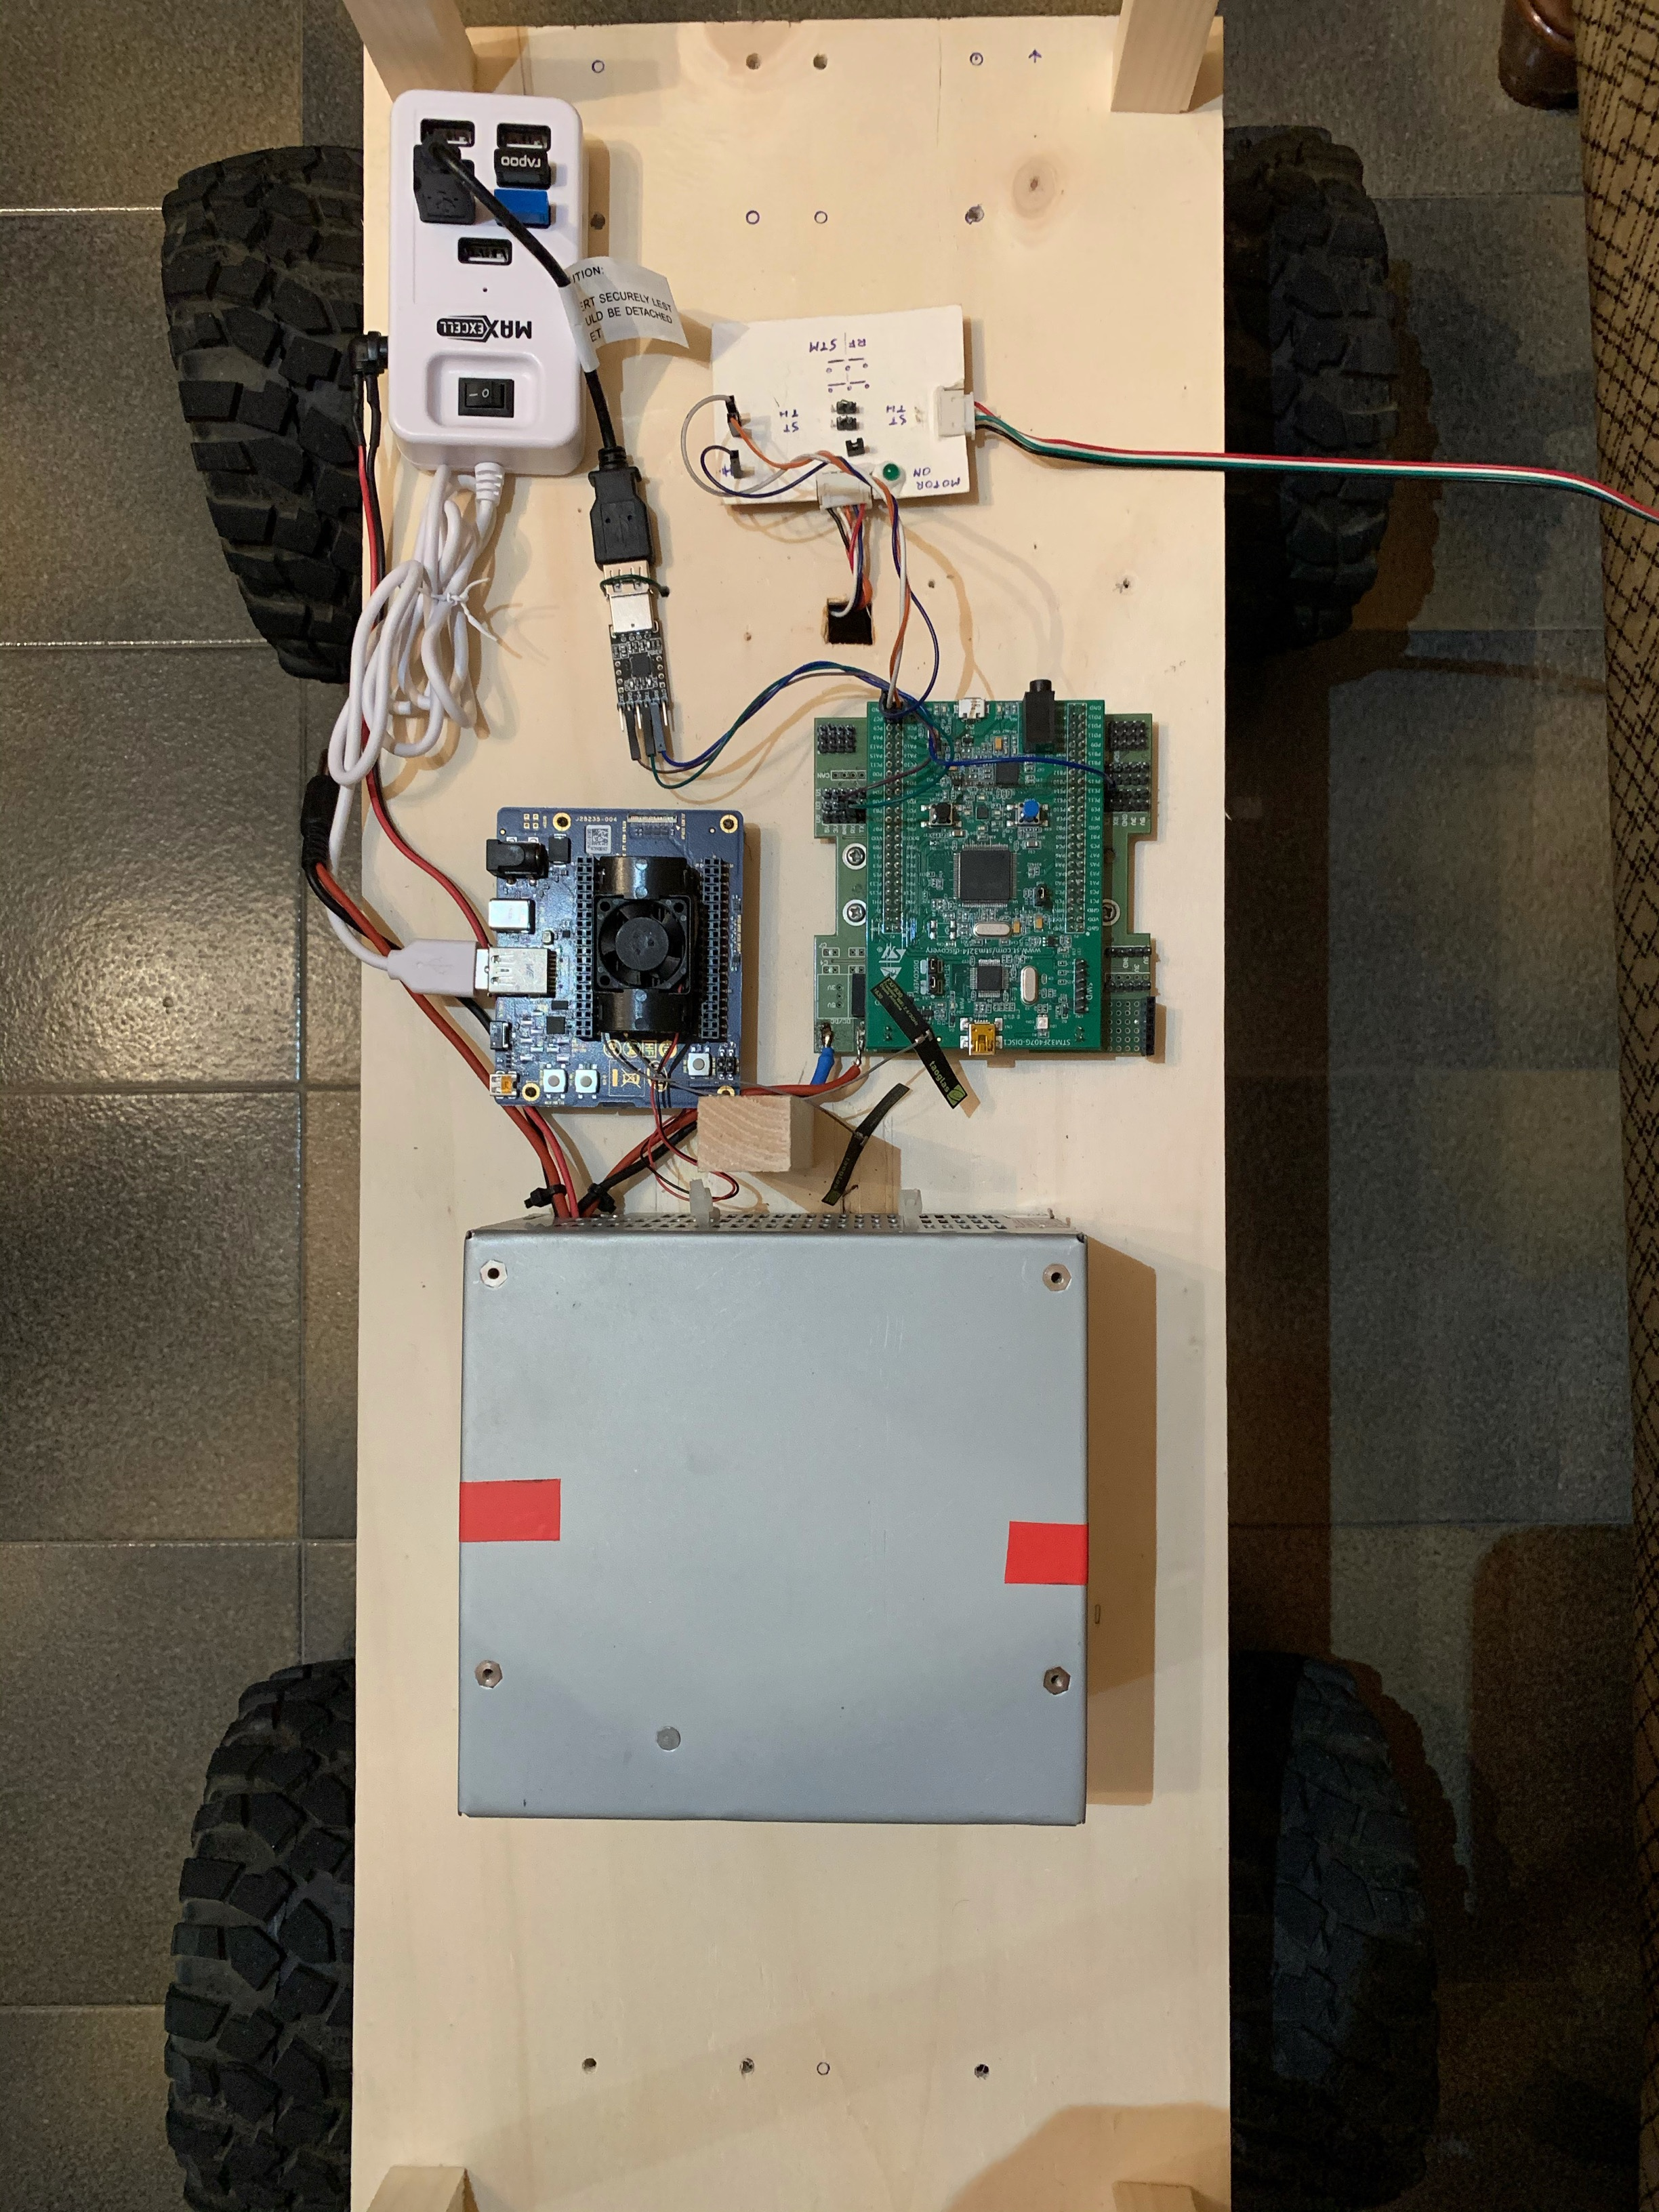
\includegraphics[width=\textwidth]{Capitolo1/Figs/foto_dopo.png}
    \caption{Foto dopo}
    \label{fig:foto_dopo}
  \end{subfigure}            
  \caption[Confronto prima e dopo cablaggio]{Confronto del cablaggio prima e dopo}
  \label{fig:confronto_cablaggio}
\end{figure}

Si è poi proceduto ad un rifacimento totale dei cablaggi, dato che era presente un disordine eccessivo, con cambi di colorazione, svariate giunzioni e connessioni parziali.

Per raggiungere un livello di ordine maggiore e migliorare la facilità di assemblaggio sono state adottate delle piattine a 5 fili per le connessioni ed è stata sviluppata anche una piccola PCB che consente di utilizzare, alternativamente all’STM\textsuperscript\textregistered, un radiocomando per il controllo di sterzo e acceleratore (vedi Figura~\ref{fig:confronto_cablaggio}).

\bigskip

La piccola PCB prodotta (Figura~\ref{fig:pcb}) ha un led di stato verde che notifica quando l’alimentazione dei motori è attiva; inoltre sono presenti due jumper che permettono di scegliere tra STM\textsuperscript\textregistered e radiocomando come sorgente del controllo per sterzo e acceleratore. Sono sempre disponibili all’utente i contatti per potersi connettere e tramite telemetria leggere quanto prodotto dal radiocomando.

\begin{figure}[h] 
\centering    
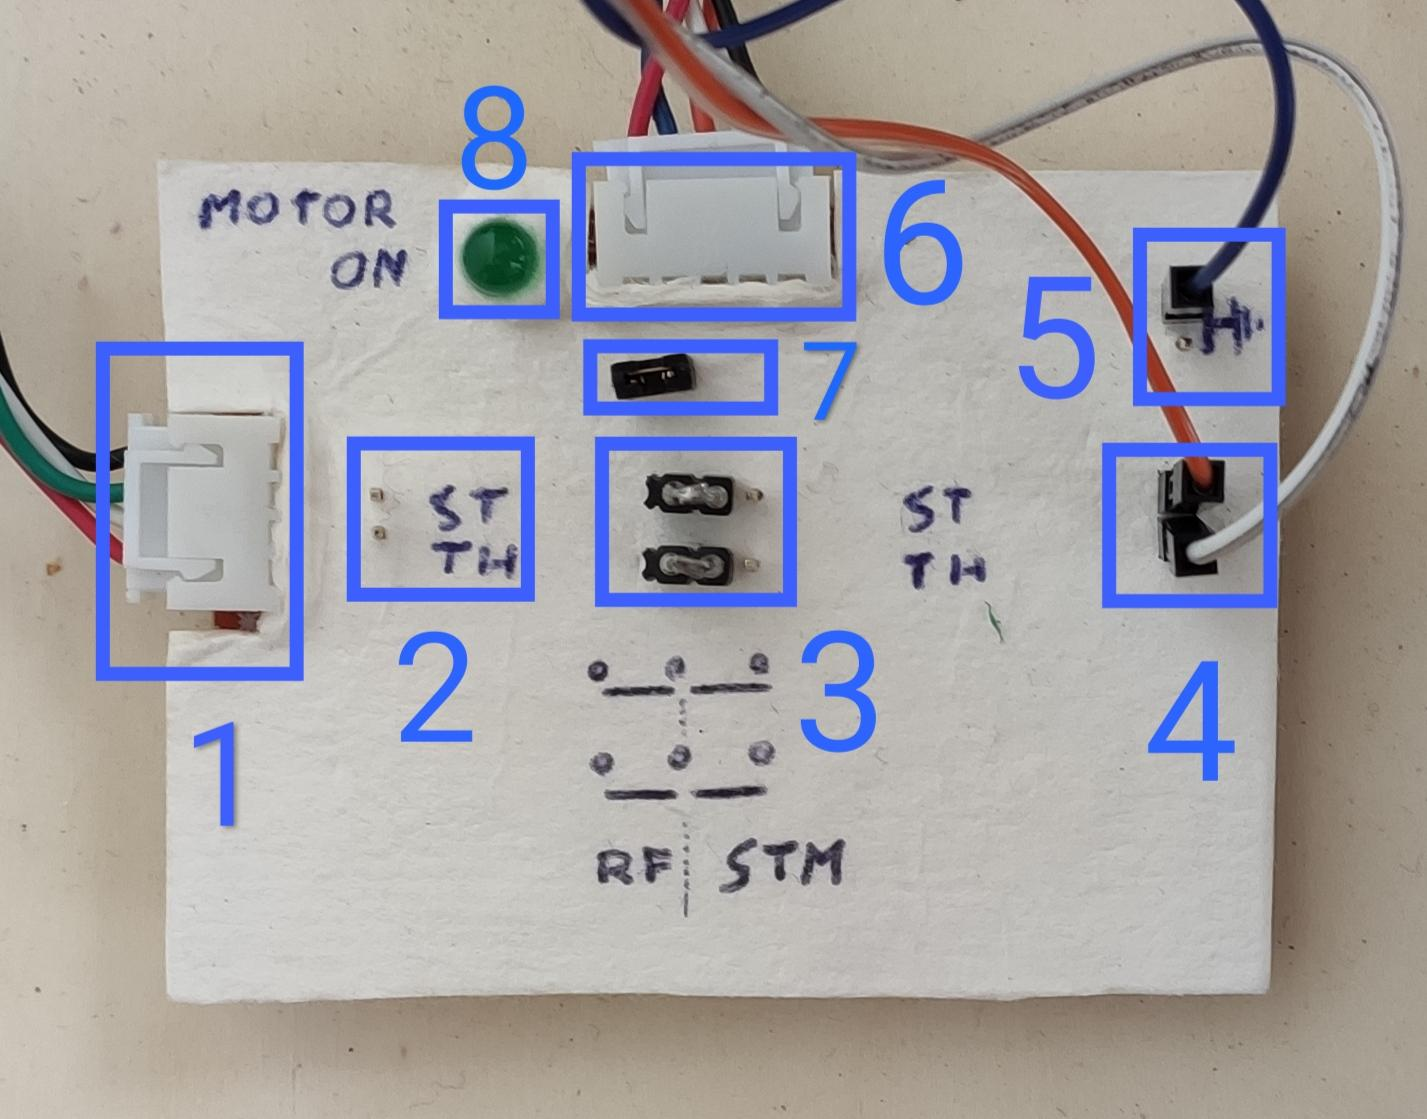
\includegraphics[width=0.45\textwidth]{Capitolo1/Figs/pcb.png}
\caption[PCB realizzata]{PCB realizzata}
\label{fig:pcb}
\end{figure}
\begin{enumerate}
    \item Connettore per il ricevitore del radiocomando;
    \item Pin per prelievo segnali PWM (steering/throttle) provenienti dal radiocomando;
    \item Jumper di selezione per la fonte di controllo: (jumper a sinistra) controllo da radiocomando e (jumper a destra) controllo da STM;
	\item Pin per connessione dei canali PWM provenienti da STM\textsuperscript\textregistered\hspace{1mm}(steering/throttle);
    \item Pin per connessione GND comune;
    \item Connettore per i motori;
    \item Jumper di abilitazione alimentazione motori;
    \item LED di stato, indica quando l'alimentazione dei motori è attiva.
\end{enumerate}

Per risolvere il problema di sottoalimentazione dei sensori è stato acquistato un HUB-USB con possibilità di alimentazione esterna; è stato quindi aggiunto un convertitore DC-DC nella scheda di alimentazione per avere a disposizione una linea a 5V, a cui è stato connesso un cavo con apposito spinotto, per permettere l’alimentazione dell’HUB-USB dalla batteria.

\bigskip

Per quanto riguarda la struttura meccanica, la durezza delle sospensioni è stata aumentata al massimo possibile, riducendo sensibilmente l’inclinazione del veicolo in curva.

\bigskip

Anche la struttura di supporto dell’elettronica è stata completamente rivista giungendo ad un rifacimento totale: infatti, a seguito della scoperta dell’interferenza elettromagnetica sulle tag da parte della sezione di alimentazione, si è scelto di disporre i sensori su un livello separato rispetto a quello delle schede di controllo e di alimentazione.
Pertanto, è stata adottata una nuova struttura in compensato, che si sviluppa su due piani paralleli disposti a $10$cm di distanza; al livello più basso si trovano Intel\textsuperscript\textregistered Joule\texttrademark \hspace{1mm}ed STM\textsuperscript\textregistered, con la scheda di alimentazione che è stata schermata inserendola all’interno di un box metallico, mentre al livello superiore vi è il Lidar in posizione centrale, e le due tag disposte lateralmente. Tutte le batterie adesso si trovano al di sotto del piano in compensato, così da concentrare il peso del veicolo in basso, ottenendo un baricentro più favorevole.

\bigskip

\begin{figure}[h] 
\centering    
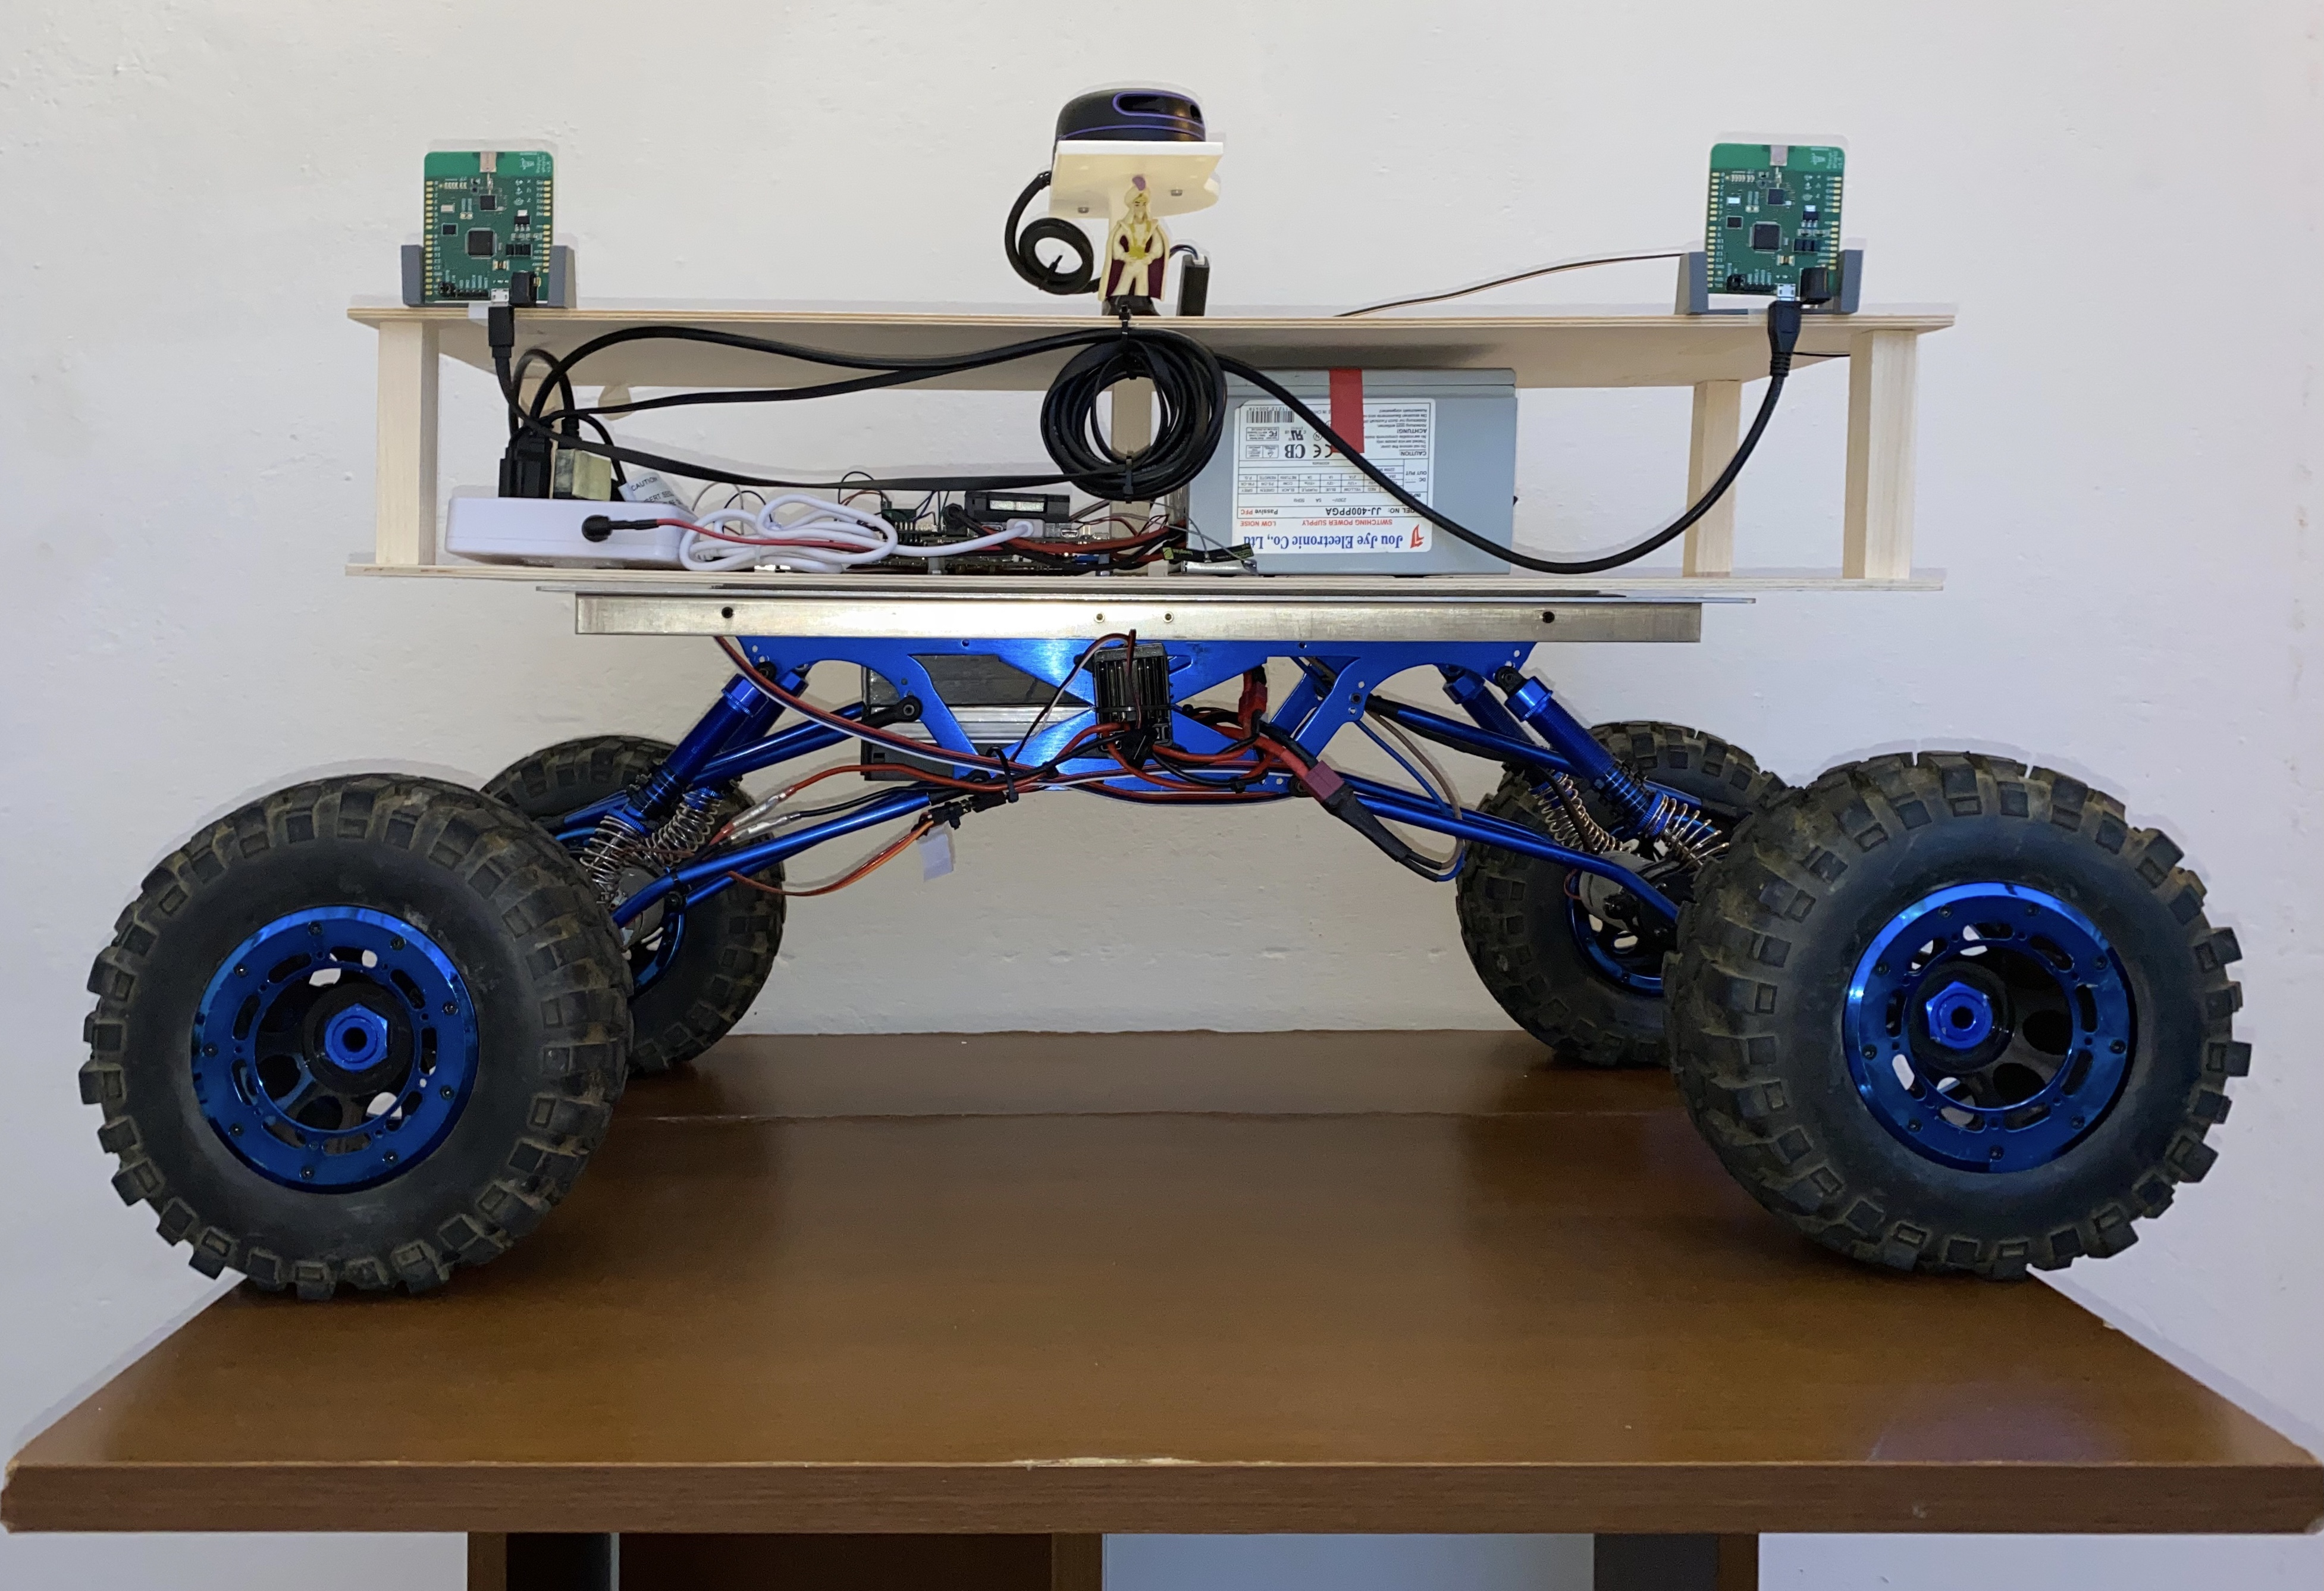
\includegraphics[width=0.77\textwidth]{Capitolo1/Figs/charlie.png}
\caption[Veicolo finale]{Veicolo Finale}
\label{fig:veicolo_finale}
\end{figure}